%deve ter coisa repetida. q bosta!
\documentclass[12pt,a4paper]{article}
\usepackage{amssymb}  %mathbb
\usepackage{amsmath}  %align
\usepackage{amsthm}   %newtheorem
\usepackage{hyperref} %a href
\usepackage{graphicx} %jpg
\usepackage[a4paper,top=1.3cm,bottom=1.3cm,left=1.3cm,right=1.3cm]{geometry}
\pagestyle{headings}
\title{Matem\'atica e Espiritualidade}
\date{}
\begin{document}
	\maketitle

	\tableofcontents
	\addtocontents{}{\protect\rule{\textwidth}{.2pt}\par}

	\section{Pre\^ambulo | Por que resolvi mostrar a face aos EUA}
			\begin{flushright}
			\end{flushright}

		Crimes contra mim s\~ao cometidos continuamente.

		Difama\c{c}\~ao. Pol\'icia. Advogado. Gravar. Fitas k7 s\~ao uma bosta. C\^ameras. Contra clarivid\^encia, nada funciona. Sabotagem. N\~ao \'e no DERCIFE. Invas\~ao. Terra sem lei. STF. M\'idia.

		Fosse tudo ideal $ \Rightarrow $ eu venderia meu peixe e pronto. No m\'aximo divulgaria livro, etc. Mas desse jeito ae, s\'o indigna\c{c}\~ao! Mosca gigante \emph{sem asas} ultrapassando as fronteiras\cite{x}.%mus

		Voc\^es v\~ao me deixar bem quietinho, sem discutir quem eu n\~ao sou? Ent\~ao... Vem a\'i a Uni\~ao Europeia!

		\begin{center}
		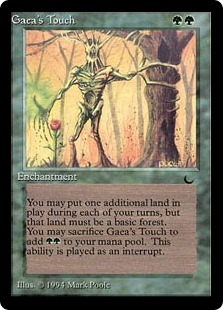
\includegraphics{gaea}
		
\includegraphics{tiosam}
		
\includegraphics{adams}
		\end{center}

		\emph{s'il vous pla�t}\cite{x}%humor

		%bom combate
		Enquanto ningu\'em fizer nada, vou ficar aqui enraivando\cite{x}. Que tal apela\c{c}\~ao? O poder paralelo, cujos interesses s\~ao o crime\cite{x} e a anarquia. Por que n\~ao fazem nada? A go\'ecia, interessada no sofrimento, por que n\~ao ridiculariza os demonistas?

	\section{Em que acredito}
			\begin{flushright}
			\end{flushright}

		$ \alpha_\omega $ \'e $ \infty $ em Amor, Justi\c{c}a e Miseric\'ordia. Jesus Cristo \'e o Mestre dos Reis Magos, por\'em os chamados \textquotedblleft milagres\textquotedblright\, est\~ao contidos em uma lei universal.

		O grande tesouro deve estar no submundo do Vaticano: todas as ideias, vislumbres e verdades reprimidas.

	\subsection{Pentateuco}
			\begin{flushright}
			\end{flushright}

\cite{ese}, cap 4, item 9. Esp(homem) foss criado com o corpo $\Rightarrow$ saber\'iamos de onde veio

Logo, Preexist\^encia da alma $\Rightarrow$ pluralidade das exist\^encias

			\begin{flushright}
			\end{flushright}

\cite{ese}, cap 4, item 13. reviver\~ao $\Rightarrow$ ressuscitar\~ao $\Rightarrow$ nega\c{c}\~ao das penas eternas $\Rightarrow$ regenera\c{c}\~ao moral

\cite{ese}, cap 4, item 16. Negar reencarna\c{c}\~ao $\Rightarrow$ negar Cristo

\cite{ese}, cap 4, item 17. O movimento revela um motor prim\'ario oculto $\Rightarrow$ reencarna\c{c}\~ao oculta.

\cite{ese}, cap 4, item 22. fixado o futuro $\Rightarrow$ n\~ao existiria progresso

Logo, existe progresso $\Rightarrow$ n\~ao existe futuro definitivo

			\begin{flushright}
			\end{flushright}

\cite{ese}, cap 5, 5. Deus \'e infinitamente contra a impunidade. sem sofrimento $\Rightarrow$ sem motivo para corrigenda

impunidade $\Rightarrow$ retardo da sociedade, assim como a poligamia.

			\begin{flushright}
			\end{flushright}

\cite{le}, q. 773 a 775: relaxar os la\c{c}os de fam\'ilia $\Rightarrow$ ego\'ismo++

O Espa\c{c}o universal \'e infinito. \cite{le}, q. 35 (h\'a controv\'ersias)

O progresso \'e quase infinito. \cite{le}, q. 169

Com a certeza do porvir, os espa\c{c}os infinitos se povoam ao infinito, em parte alguma h\'a o vazio e a solid\~ao; a solidariedade liga todos os seres, aqu\'em e al\'em da tumba. A g\^enese, cap. 1, 62

			\begin{flushright}
			\end{flushright}

PAIX\~OES: \textquotedblleft Compreende a sua natureza espiritual aquele que as procura REPRIMIR.\textquotedblright\, \cite{le}, Q 911

\subsection{Humildade Edificante}
			\begin{flushright}
			\end{flushright}

Discordo veementemente e s\'o vou me calar se os esp\'iritos estiverem
positivamente contra mim, for\c{c}ando meu desencarne \textquotedblleft para evitar danos
maiores\textquotedblright. Mas eles h\~ao de concordar que:

1) Enquanto n\~ao dou conta de tecer l\~a como Paulo de Tarso, vou tentando
trabalhar de manh\~a, dar aula \`a tarde, estudar \`a noite e dormir
tranquilamente 5x/semana. muita coisa ilus\'oria, mas necess\'aria.

2) a humildade verdadeira concede o reino dos c\'eus no presente @Huberto
Rohden sobre Mateus 5, 3.

3) Se n\~ao temos o reino dos c\'eus no presente e vivenciamos raiva,
ansiedade, apego, tristeza, ressentimento, et cetera, et cetera, et
cetera, \'e porque n\~ao somos verdadeiramente humildes. Somos orgulhosos.

4) De acordo com a lei do trabalho/progresso, atrav\'es de disciplina
adquiriremos a humildade. Combatendo o orgulho interno. E talvez...

5) existam causas externas. Caso contr\'ario eu esqueceria o outro e
viveria num mundo ego\'istico, contradizendo a morte do ego em Mateus 5,
4.

6) Ao inv\'es do esquecer, coloquemos perdoar. (O texto fala sem
exig\^encia.) Compreender.

7) At\'e agora s\'o compreendo que a maldade alheia \'e resultado do
sofrimento alheio. Sofremos por diferentes raz\~oes, at\'e...

8) viver a lei de igualdade. Nem acima, nem abaixo do outro.

9) Para todo aquele dentro de que houver firmeza interior, n\~ao racional,
 mas profunda, no n\'ivel do Ser Espiritual, o reino dos c\'eus \'E uma
realidade tang\'ivel, ainda que a carca\c{c}a do ser esteja pregada na cruz,
ou coisa pior.

	\section{Axiomas}
			\begin{flushright}
			\end{flushright}

		AMAI.

		Educai-vos, instru\'i-vos.

		$ \alpha_\omega $ \'e infinitamente amor/bondade.

		\textquotedblleft Em verdade, em verdade...\textquotedblright\, = Realidade espiritual. Em oposi\c{c}\~ao \`a ilus\~ao\cite{x} da mat\'eria.

	\subsection{Trechos}
			\begin{flushright}
			\end{flushright}

\textquotedblleft N\'os somos agora o resultado do que pensamos at\'e hoje.\textquotedblright\, Lucidez, p. 139

			\begin{flushright}
			\end{flushright}

\textquotedblleft Se sou humilde, nunca me sentirei humilhado. / Se me sinto humilhado, humilde n\~ao sou.\textquotedblright\, Rindo e Refletindo com Chico Xavier, vol. 2, p. 116

			\begin{flushright}
			\end{flushright}

\textquotedblleft Muitos irm\~aos, ao vivenciarem estados infelizes em seu passado espiritual, quando pelos seus atos feriram deliberadamente a vida do pr\'oximo, com escolhas que desafiaram a lei divina, intentaram esconder o ato infeliz, alojando suas lembran\c{c}as nas zonas mais profundas do psiquismo. Por\'em, os reflexos de suas a\c{c}\~oes se mostram pelo remorso que remoem em seu \'intimo, ou em outras fases do pensamento doentio, sabendo que n\~ao podem enganar os postulados da divina lei. / Estes reveses do passado, ao emergirem da subconsci\^encia mental, manifestam|se nas psicoses, nas neuroses e em muitos casos de esquizofrenia, que s\~ao diagnosticados por meus irm\~aos (...) da ci\^encia terrena.\textquotedblright\, Medicina da Alma, p. 146

			\begin{flushright}
			\end{flushright}

\textquotedblleft Se algu\'em te fere com uma simples palavra, ainda n\~ao ficaste livre das enfermidades do orgulho e da vaidade, do ego\'ismo e da vingan\c{c}a. / Aprenda a discernir o que vem por tr\'as das ofensas e as li\c{c}\~oes que poder\'as receber delas. Se bem compreendidas, \'e Deus que Se faz presente e mais vis\'ivel em teu cora\c{c}\~ao.\textquotedblright\, Cirurgia Moral, p. 23

			\begin{flushright}
			\end{flushright}

A Educa\c{c}\~ao(ser). \textquotedblleft A vis\~ao unit\'aria entre natureza humana e leis morais, entre virtude e satisfa\c{c}\~ao da alma, afasta o conflito entre o ser e o dever|ser. Entre esses dois p\'olos, existe apenas um processo | o da educa\c{c}\~ao, entendida como um despertar, um tornar|se consciente de. / Tamb\'em a rela\c{c}\~ao entre conhecimento e virtude faz do mal uma conting\^encia da ignor\^ancia. N\~ao h\'a perversidade natural, mas apenas inconsci\^encia\cite{Freud} do verdadeiro bem.\textquotedblright\, Pedadogia Esp\'irita, p. 99 INCONTRI

			\begin{flushright}
			\end{flushright}

\textquotedblleft Quem mais serve, por amor, \'e quem mais \'e capaz de fazer brotar o impulso do bem na alma humana. Quem mais se sacrifica, por amor, \'e quem mais alcan\c{c}a a intimidade do outro, para faz\^e|lo melhor.\textquotedblright\, Pedagogia Esp\'irita, p. 118

			\begin{flushright}
			\end{flushright}

\textquotedblleft Ser\'a que sua viv\^encia atual (...) \'e um produto necess\'ario a seu desenvolvimento e crescimento espiritual, ou simplesmente fruto de uma autopuni\c{c}\~ao ou de um auto-engano?\textquotedblright\, A Imensid\~ao dos Sentidos, p. 184

			\begin{flushright}
			\end{flushright}

\textquotedblleft Quem serve por amor ao servi\c{c}o e tem a Deus por Pai e Jesus por irm\~ao, n\~ao pode deter|se para informar|se sobre o que pensam os homens ao seu respeito...\textquotedblright\, O Abismo, p. 56

			\begin{flushright}
			\end{flushright}

Sempre que se te enseje oportunidade de servir, de construir, de auxiliar, de olvidar os preju\'izos que te hajam causado, n\~ao te detenhas ante o prazer de realiz\'a|los, disputando a honra de ser aquele que sempre est\'a \`a disposi\c{c}\~ao de todos na aduana da fraternidade. // Os teus atos s\~ao os teus acusadores ou defensores no tribunal de tua consci\^encia e te representar\~ao diante da Legisla\c{c}\~ao Divina. (Joanna de Angelis, Nascente de B\^en\c{c}\~aos, p. 121)

	\section{Existe uma penalidade suprema.} %penas e gozos
			\begin{flushright}
			\end{flushright}

		Lema: Toda penalidade \'e finita.

		Se $ \alpha_\omega $ tivesse criado seres sem saber que seriam condenados eternamente, n\~ao seria onisciente, se os criou sabendo disso, n\~ao seria infinitamente bom e justo. (Pedagogia Esp\'irita\cite{x}, p. 168)

		Cuidado: um milh\~ao de anos \'e tempo finito.

		Ou seja, se houvesse um inferno, haveria sofrimento $ \infty $. Ent\~ao, $ \alpha_\omega $ seria infinitamente mau.

		Considere o conjunto de todas as penalidades aplicadas. $\exists$ um maior elemento.

		Caso contr\'ario, a cada penalidade aplicada, haveria outra maior.

		Assim, haveria uma penalidade t\~ao grande quanto se quisesse. Q.E.A.\cite{x}

		\emph{\^o, evolu\'idos!? eu tou querendo saber agora quem foi o cara e qual foi a maior penalidade aplicada na eternidade da Cria\c{c}\~ao.}

	\section{A ess\^encia de tudo est\'a no AMAI}
		\begin{flushright}
		\end{flushright}

		Mandamentos de Jesus Cristo, o Mestre Verdadeiramente Libertador:

		$\mathbb{AMAI}$. A $ \alpha_\omega $. A Si. ao Pr\'oximo. Com equil\'ibrio. Lucas 10, 27 \cite{x}

		\textquotedblleft Amai-vos como eu vos amei.\textquotedblright\, Jo\~ao 13, 34

		\textquotedblleft Amai aos vossos inimigos.\textquotedblright\, Mateus 5, 44

		\textquotedblleft Sede perfeitos, como o Pai Celestial o \'e.\textquotedblright\, Mateus 5, 48


	\section{Verdades}
		\begin{flushright}
		\end{flushright}

		\textquotedblleft Conhecereis a Verdade, e a Verdade vos Libertar\'a.\textquotedblright\, Jo\~ao 8, 32.

		Ainda estou vendo verdades no externo. E estou mergulhado em uma infinidade de falsidades mais aceitas que 1 + 2 = 3. Esse papo de conhecereis a verdade parece ser o c\'umulo do b\'asico. Estou vendo explora\c{c}\~ao por toda parte, tamb\'em. \textquotedblleft Vamos explorar o Brasil. Vamos explorar a China.\textquotedblright\, Gastam at\'e a destrui\c{c}\~ao. O que tem mais: explora\c{c}\~ao ou falsidade? Ser\'a que o mundo vai consumir a Verdade chinesa contida numa tirinha de papel?

		Redefini\c{c}\~oes:

		\subsection{Verdadeiro caminho}
			\begin{flushright}
			\end{flushright}

			\textquotedblleft Ningu\'em... ningu\'em vem ao Pai Celestial... sen\~ao por mim.\textquotedblright

			\textquotedblleft Eu sou o Caminho, a Verdade e a Vida.\textquotedblright\, Jo\~ao 14, 6.

			Jesus \'e o caminho\cite{x} at\'e a Perfei\c{c}\~ao\cite{x}.

		\subsection{Verdadeira coragem}
			\begin{flushright}
			\end{flushright}

			A verdadeira coragem n\~ao est\'a na decis\~ao escandalosa de um dia, mas no sagrado cumprimento dos votos empenhados para uma vida inteira. (Ren\'uncia\cite{x}, de Francisco C\^andido Xavier)

			A coragem de ser crist\~a(o). Voc\^e tem? Este s\'o faz o bem e n\~ao se omite. N\~ao s\'o nos atos, mas tamb\'em em pensamentos e palavras.

		\subsection{Verdadeira fam\'ilia}
			\begin{flushright}
			\end{flushright}

			Sangue \'e ilus\~ao.

			Marcos 3, 20.21.31-35; Mateus 12, 46-50 (\cite{ese}, cap. 14, item 5)

		\subsection{Verdadeira liberdade, ou perfei\c{c}\~ao\cite{x}}
			\begin{flushright}
			\end{flushright}

			Ser verdadeiramente livre $ \Rightarrow $ Ser o que verdadeiramente se \'e \cite{x}. (Kierkegaard) %deus interno

			Ser livre da mat\'eria\cite{x}, das ilus\~oes\cite{x}, de tudo o que \'e imperfeito, implica ser uno\cite{x} com o Todo.

			O caminho\cite{x}, a salva\c{c}\~ao, a liberta\c{c}\~ao est\'a na educa\c{c}\~ao da alma.

			Qual \'e o pr\'oximo passo?

	\section{Ora\c{c}\~oes}
			\begin{flushright}
			\end{flushright}

		\subsection{Prece de C\'aritas}
			\begin{flushright}
			\end{flushright}

			Deus, nosso Pai, que sois todo poder e bondade,

			dai for\c{c}a \`aquele que passa pela prova\c{c}\~ao,

			dai luz \`aquele que procura a verdade,

			ponde no cora\c{c}\~ao do homem a compaix\~ao e a caridade.

			Deus! Dai ao viajor a estrela-guia, ao aflito a consola\c{c}\~ao, ao doente o repouso.

			Pai! Dai ao culpado o arrependimento, ao esp\'irito a verdade, \`a crian\c{c}a o guia, ao \'orf\~ao o pai.

			Senhor! Que a vossa bondade se estenda sobre tudo que criaste.

			Piedade, Senhor, para aquele que vos n\~ao conhece, esperan\c{c}a para aquele que sofre.

			Que vossa bondade permita aos esp\'iritos consoladores derramarem por toda parte a paz, a esperan\c{c}a e a f\'e.

			Deus! Um raio, uma fa\'isca do vosso amor pode abrasar a terra;

			deixai-nos beber nas fontes dessa bondade fecunda e infinita

			e todas as l\'agrimas secar\~ao, todas as dores acalmar-se-\~ao,

			um s\'o cora\c{c}\~ao, um s\'o pensamento subir\'a at\'e V\'os, como um grito de reconhecimento e de amor.

			Como Mois\'es sobre a montanha, n\'os vos esperamos com os bra\c{c}os abertos.

			Oh! Poder. Oh! Bondade. Oh! Beleza. Oh! Perfei\c{c}\~ao.

			E queremos de algum modo alcan\c{c}ar/merecer a Vossa miseric\'ordia.

			Deus! Dai-nos a for\c{c}a de ajudar o progresso a fim de subirmos at\'e V\'os:

			dai-nos a caridade pura, dai-nos a f\'e e a raz\~ao,

			dai-nos sobretudo a simplicidade

			que far\'a das nossas almas espelho

			onde se refletir\'a a vossa imagem.

		\subsection{Ora\c{c}\~ao de S\~ao Francisco de Assis}
			\begin{flushright}
			\end{flushright}

			Senhor,

			Fazei-me instrumento de vossa paz.

			Onde houver \'odio, que eu leve o amor,

			Onde houver ofensa, que eu leve o perd\~ao.

			Onde houver disc\'ordia, que eu leve a uni\~ao.

			Onde houver d\'uvida, que eu leve a f\'e.

			Onde houver erro, que eu leve a verdade.

			Onde houver desespero, que eu leve a esperan\c{c}a.

			Onde houver tristeza, que eu leve a alegria.

			Onde houver trevas, que eu leve a luz.

			\'O Mestre,

			Fazei que eu procure mais

			Consolar, que ser consolado.

			Compreender, que ser compreendido.

			Amar, que ser amado.

			Pois \'e dando, que se recebe.

			\'E perdoando, que se \'e perdoado

			E \'e morrendo, que se vive

			Para a vida eterna.

		\subsection{Prece Diante da Natureza}
			\begin{flushright}
			\end{flushright}

			Senhor da Vida!

			diante da Natureza,

			manifesta\c{c}\~ao incontest\'avel da tua cria\c{c}\~ao,

			permite que os homens se re\'unam em ora\c{c}\~ao

			louvando a naturalidade das coisas...

			Pai de infinita bondade, faze com que eles possam aprender:

			. com a sensibilidade das flores, exalar o perfume do bom senso;

			. com o amparo e o resguardo das \'arvores, criar ra\'izes de resist\^encia diante dos obst\'aculos;

			. com a quietude das montanhas, serenidade para fazer auto-observa\c{c}\~ao;

			. com a musicalidade das aragens, entender a harmonia das leis da vida;

			. com a tranquilidade dos lagos, refletir sobre o potencial interior;

			. com a determina\c{c}\~ao dos rios que buscam o seio dos mares, sedimentar o poder de realiza\c{c}\~ao;

			. com a espontaneidade dos p\'assaros, dar asas \`a criatividade;

			. com a estrutura fecunda do solo que nos proporciona frutos, ser receptivos \`as boas ideias;

			. com a simplicidade dos brotos nos ramos f\'erteis, ser flex\'iveis \`as novas concep\c{c}\~oes;

			. com os frutos da terra, abastecer o celeiro da alma.

			Podemos notar, Soberano do Universo, que a Natureza estabelece o equil\'ibrio das cria\c{c}\~oes e das criaturas atrav\'es das tuas leis naturais, e a n\'os cabe observ\'a-la para que possamos viver com ordem, aux\'ilio m\'utuo e modera\c{c}\~ao.

			Ante as dificuldades, Senhor, que os homens possam ser como a \'agua, que em sil\^encio adapta-se \`as limita\c{c}\~oes que os teus des\'ignios imp\~oem atrav\'es da Natureza, mas que prossegue em frente, contornando de maneira equilibrada os empecilhos que encontra pelo caminho.

			Estamos cientes, Pai, de que as leis naturais mostram como tudo acontece, e observar a naturalidade das coisas pode ser um educador bem mais confi\'avel do que os livros e palavras dos seres humanos, pois, conforme os s\'abios asseguram, \textquotedblleft a Natureza \'e a arte de Deus\textquotedblright.

			Alma do Universo, guarda-nos em tua paz.

			N\~ao s\'o agora, mas para todo o sempre.

			Que assim seja.

			Francisco do Esp\'irito Santo Neto, por Hammed

			Lucidez

			30

	\section{Na Presen\c{c}a do Amor}
		\begin{flushright}
		\end{flushright}

		\textquotedblleft Aquele que ama a seu irm\~ao est\'a na luz e nele n\~ao h\'a esc\^andalo.\textquotedblright\, Jo\~ao. (I Jo\~ao 2, 10)

		Quem ama o pr\'oximo sabe, acima de tudo, compreender. E quem compreende sabe livrar os olhos e ouvidos do venenoso visco do esc\^andalo, a fim de ajudar, ao inv\'es de acusar ou desservir.

		\'E necess\'ario trazer o cora\c{c}\~ao sob a luz da verdadeira fraternidade, para reconhecer que somos irm\~aos uns dos outros, filhos de um s\'o Pai.

		Enquanto nos demoramos na escura fase do apego exclusivo a n\'os mesmos, encarceramo-nos no ego\'ismo e exigimos que os outros nos amem. Nesse passo infeliz, n\~ao sabemos querer sen\~ao a n\'os pr\'oprios, tomando os semelhantes por instrumentos de nossa satisfa\c{c}\~ao.

		Mas se realmente amamos os companheiros de caminho, a paisagem de vida se modifica, de vez que a claridade do amor nos banhar\'a a vis\~ao.

		Ama, pois, e assim como a lama jamais ofende a luz, a ofensa n\~ao mais te alcan\c{c}ar\'a.

		Saber\'as que a mis\'eria \'e fruto da ignor\^ancia e auxiliar\'as a v\'itima do mal, nela encontrando o pr\'oprio irm\~ao necessitado de apoio e entendimento.

		Aprender\'as a ouvir sem revolta, ainda mesmo que o crime te procure os ouvidos, e cultivar\'as a ajuda ao advers\'ario, ainda mesmo quando te vejas dilacerado, porque o perd\~ao com esquecimento absoluto dos golpes recebidos surgir\'a espont\^aneo em teu esp\'irito, assim como a toler\^ancia aparece natural na fonte que acolhe no pr\'oprio seio as pedras que lhe atiram.

		Ama e compreender\'as.

		Compreende e servir\'as sempre mais cada dia, porque ent\~ao permanecer\'as sob a gl\'oria da luz, inacess\'ivel a qualquer incurs\~ao das trevas.

		Francisco C\^andido Xavier, por Emmanuel

		Fonte Viva

		159

	\section{Ante a Luz da Verdade}
		\begin{flushright}
		\end{flushright}

		\textquotedblleft Conhecereis a verdade e a verdade vos libertar\'a.\textquotedblright\, | Jesus. (Jo\~ao 8, 32)

		A palavra do Mestre \'e clara e segura.

		N\~ao seremos libertados pelos \textquotedblleft aspectos da verdade\textquotedblright\, ou pelas \textquotedblleft verdades provis\'orias\textquotedblright\, de que sejamos detentores no c\'irculo das afirma\c{c}\~oes apaixonadas a que nos inclinemos.

		Muitos, em pol\'itica, filosofia, ci\^encia e religi\~ao, se afei\c{c}oam a certos \^angulos da verdade e transformam a pr\'opria vida numa trincheira de luta desesperada, a pretexto de defend\^e-la, quando n\~ao passam de prisioneiros do \textquotedblleft ponto de vista\textquotedblright.

		Muitos aceitam a verdade, estendem-lhe as li\c{c}\~oes, advogam-lhe a causa e proclamam-lhe os m\'eritos, entretanto, a verdade libertadora \'e aquela que conhecemos na atividade incessante do Eterno Bem.

		Penetr\'a-la \'e compreender as obriga\c{c}\~oes que nos competem.

		Discerni-la \'e renovar o pr\'oprio entendimento e converter a exist\^encia num campo de responsabilidade para com o melhor.

		S\'o existe verdadeira liberdade na submiss\~ao ao dever fielmente cumprido.

		Conhecer, portanto, a verdade \'e perceber o sentido da vida.

		E perceber o sentido da vida \'e crescer em servi\c{c}o e burilamento constantes.

		Observa, desse modo, a tua posi\c{c}\~ao diante da Luz...

		Quem apenas vislumbra a gl\'oria ofuscante da realidade, fala muito e age menos. Quem, todavia, lhe penetra a grandeza indefin\'ivel, age mais e fala menos.

		Francisco C\^andido Xavier, por Emmanuel

		Fonte Viva

		173

	\section{Bot\^anica}
			\begin{flushright}
			\end{flushright}

		Flor de L\'otus \href{http://en.wikipedia.org/wiki/Victoria_(waterlily)}{brasileira}

	\section{Teoria da Bosta}
			\begin{flushright}
			\end{flushright}

		Assim como o organismo se livra dos despojos, jogando para o externo em forma de excre\c{c}\~ao, o corpo espiritual se despoja de seus males, jogando-os para o corpo f\'isico\cite{x} em forma de doen\c{c}as.

	\section{Continuidade}
			\begin{flushright}
			\end{flushright}

		\emph{| Morreu, acabou.}

		Botou o ovo, acabou? Caiu o fruto, acabou? Caiu a bosta, acabou? Gozou, acabou? Portanto, continuemos.

  	\section{\emph{Unfiled}}
			\begin{flushright}
			\end{flushright}

			Consequ\^encias de Peano. $2 + 2 \rightarrow x \neq 4$, desde que se conserve outra coisa.

			\emph{| Tem que ter crime, sen\~ao n\~ao tem \textquotedblleft gra\c{c}a\textquotedblright.}

			Ci\^encia medi\'unica: \# m\'ediuns $\rightarrow \infty \Rightarrow$ mesma informa\c{c}\~ao.

			Psicologia: mesmas experi\^encias, resultados diferentes. \# CNTP $\Rightarrow$ mesmo resultado sobre a natureza humana.

			Fui comparado a uma mulher gostosa que \emph{pode\cite{x} ter qualquer homem que quiser}. Faltou acrescentar: superficialmente, pra variar. Bom, eu nunca vi uma mulher dizendo bora l\'a em casa huahuahuahua nem nada profundo o bastante.

			Eu curto o furo da Dani Calabresa. Teve uma a cara dela que tentou me incriminar. Ai que saudades das pomadas.

			Mataram o Eneas com doen\c{c}a rara e para mim n\~ao d\~ao inje\c{c}\~ao letal quando pe\c{c}o. \emph{Long long time... Voc\^e est\'a muito desesperan\c{c}ado.}

			Estou sendo acusado perante o capeta de ser ele e ele s\'o ri.

			\emph{Long long time...} Aquela tal de Maria Eugenia ficava chamando os alunos de orangotango e pelo que lembro comigo foi s\'o pelas costas. Olha s\'o! A evolu\c{c}\~ao j\'a est\'a no senso comum: o orangotango vira homem! Com ela quase que eu ca\'i na modalidade pontua\c{c}\~ao il\'icita.

			Cumpra-se ou rasgue-se a lei? \emph{Long long time...} | O que n\'os estamos fazendo aqui??? | \'E o empregador, que n\~ao cumpriu sua parte.

			Internet na conta de luz! Frequ\^encias moduladas! Seja o universo verdadeiro uma onda portadora e o nosso somente uma fase. A verdade \'e trif\'asica? he

			CNJ do mal quer economizar com um turno de 8h/d ao inv\'es de dois turnos de 6h/d. Deveria era ter o coordenador da manh\~a e o coordenador da tarde, o gerente da manh\~a e o gerente da tarde, o diretor da manh\~a e o diretor da tarde. Mas eles n\~ao podem falar que est\~ao cansados. Diunvirato j\'a!

			Ou eu concordo, ou eu saio fora. E a pessoa que vai \`a igreja e concorda es\'a meio desesperada.

			\begin{flushright}
			\end{flushright}

			Cada ser humano \'e uma inc\'ognita a ser equacionada por ele pr\'oprio. (Autodescobrimento, 42)

			Nos podem for\c{c}ar a \textquotedblleft ser escravos\textquotedblright, mas n\~ao nos podem for\c{c}ar a \textquotedblleft ser livres\textquotedblright. (Os Prazeres da Alma, 123)

			Da mesma forma que n\~ao podemos protestar ou lutar contra os ecos que ressoam pelo efeito de nossos pr\'oprios ru\'idos ou palavras, igualmente n\~ao devemos ralhar com as pessoas ou fatos da vida dom\'estica, pois s\~ao somente reflexos da realidade interior, atra\'idos e materializados pelo nosso estado de consci\^encia. (154)

			O orgulhoso utiliza unicamente o que sup\~oe ou imagina, n\~ao o que sente. Sua percep\c{c}\~ao \'e distorcida, pois ele apenas d\'a import\^ancia ao que os outros v\~ao pensar ou achar dele e n\~ao presta aten\c{c}\~ao em seu \textquotedblleft universo interior\textquotedblright. Ele vive apenas \textquotedblleft experi\^encias teatrais\textquotedblright\, | interpreta pap\'eis no \textquotedblleft palco da vida\textquotedblright. (A Imensid\~ao dos Sentidos, 68)

			Quem ama se torna, gradativamente, um indiv\'iduo pleno; por isso, nem sempre \'e conveniente aos tiranos e dominadores nos incentivar ao amor. N\~ao nos querem libertos, originais e criativos. (180)

			N\~ao \`a gl\'oria em sofrer por sofrer! N\~ao existe nenhuma recompensa em cultuar a dor; na verdade, n\~ao estamos aqui para mostrar como temos sido padecentes, mas sim para aprendermos como cessar as amarguras que nos afligem, como crescermos espiritualmente, como superarmos nossos pontos fracos e como recuperarmo-nos dos equ\'ivocos, prosseguindo no cultivo do progresso interior, com tranquilidade e satisfa\c{c}\~ao de viver. (184)

			O homem moderno vive na ilus\~ao de saber o que quer, quando de fato ele quer o que se sup\~oe que deva querer. (Cita\c{c}\~ao de Pedagogia Esp\'irita\cite{x}, p. 79)

			Ante a Luz da Verdade

			Huberto Rohden %***

			A g\^enese da ilus\~ao: Eva mente a Ad\~ao, dizendo que era uma frutinha qualquer. Por isso, Verdade \'e yang.

			Nos animais, prevalece a Verdade. Nos homens, por consequ\^encia do livre-arb\'itrio, esta vai amadurecendo. A perfei\c{c}\~ao interna passa a conviver (muitas vezes guerrear) com a ilus\~ao externa. Quando a ilus\~ao come\c{c}a a invadir o interior... aliena\c{c}\~ao de si mesmo.

			%bom combate, mono.
			Antes de mandar algu\'em para o inferno\cite{x} at\'e a quarta gera\c{c}\~ao, tento lembrar que de maledic\^encia e viol\^encia o umbral est\'a cheio. Mais conhecido como purgat\'orio.

			um cara como eu que n\~ao bebe, n\~ao fuma, n\~ao \'e convidado para churrasco nem faz quest\~ao de pagar por isso... tenho mais \'e que pedir a $ \alpha_\omega $ para me libertar da sexualidade e voar prum mundo mais evolu\'ido.

			dizem-se crist\~aos e n\~ao t\^em atitude crist\~a. o que s\~ao? hip\'ocritas!

			\textquotedblleft Vin\'icius, seu hip\'ocrita, tira primeiro a trave do teu olho.\textquotedblright

			voc\^es est\~ao loucas s\'o porque eu estou publicando? \'e uma \textquotedblleft divulga\c{c}\~ao\textquotedblright\, do espiritismo? pois se eu estivesse 100\% feliz, para que publicaria? estou preocupado com os outros $ \Rightarrow $ \'e porque tem \textquotedblleft alguma coisa\textquotedblright\, errada ae.

			%mus
			\textquotedblleft amor\cite{x} \'e crist\~ao, sexo \'e pag\~ao\textquotedblright\cite{x}??? culpa do(s) Conc\'ilio(s)\cite{x} de Niceia

			quem ama, dissemina. voc\^e me ama e n\~ao sabe o que fazer? enfrente os servidores da ilus\~ao! %ilusao

			conjectura: o demonismo \'e um potencial destruidor da humanidade.

			\begin{flushright}
			\end{flushright}

| Estagnado.

| \'E que essas consequ\^encias s\~ao muito bomb\'asticas. Tenho medo da pr\'oxima!

\textquotedblleft realiza\c{c}\~ao que se reveste de valores morais e espirituais enfrenta incont\'aveis dificuldades que devem ser superadas. Os riscos da incompreens\~ao dos demais, das agress\~oes intempestivas dos violentos, das cal\'unias bem apresentadas por muitos, da exposi\c{c}\~ao ao rid\'iculo e da descren\c{c}a quase generalizada, constituem circunst\^ancias naturais no cotidiano da humanidade. No entanto, quem teme essas lutas, certamente n\~ao possui amadurecimento psicol\'ogico nem ideal digno de cr\'edito, porque se contenta com o convencional e j\'a realizado.\textquotedblright\, Joanna de Angelis, Divaldo Pereira Franco, Nascente de B\^en\c{c}\~aos, 2 - Autodetermina\c{c}\~ao, p. 19

			\begin{flushright}
			\end{flushright}

| o que \'e religi\~ao?

tem gente achando assiste jogos religiosamente;

tem gente que \textquotedblleft se diverte\textquotedblright\, todo fim de semana religiosamente...

			\begin{flushright}
			\end{flushright}

existe uma justi\c{c}a interna e outra externa.

na interna \textquotedblleft bem aventurados os que sofrem persegui\c{c}\~ao 'por conta' da justi\c{c}a\textquotedblright\, em Huberto Rohden. \'e a consci\^encia. maior justi\c{c}a, maior perfei\c{c}\~ao. menos auto-engano. logo amar a si.

na externa vive a rela\c{c}\~ao entre o \emph{self} e o \emph{alter}. logo amar o pr\'oximo.

e a deus?

			\begin{flushright}
			\end{flushright}

proposi\c{c}\~ao: existe um \'unico espiritismo tal que:

1) existe reencarna\c{c}\~ao

2) n\~ao admite vida mon\'astica

3) n\~ao \'e ocultista

4) n\~ao \'e polite\'ista

s\'o estava faltando isso mesmo: criticar os mon\'asticos. onde est\'a a linha que divide o cuidar de si do ego\'ismo? essa peirgunta vale a alma de um monge

			\begin{flushright}
			\end{flushright}

o amor \'e essencial e n\~ao demonstr\'avel.

			\begin{flushright}
			\end{flushright}

ilus\~oes de grandeza: meu psik est\'a achando que eu penso assim: quem \'e o cara que desvia o caminho dos outros? quem \'e o cara que est\'a constantemente no pensamento dos outros? quem \'e o importante pra todo mundo? quem faz as pessoas deixarem de viver para comentar? quem incomoda? quem \'e o mais comentado do oeste? quem \'e o cara?

			\begin{flushright}
			\end{flushright}

		| tem uma coisa muito errada nessa est\'oria.

		| simples. a maioria n\~ao tem raz\~ao.

			\begin{flushright}
			\end{flushright}

| Esse cara a gente trata igual mendigo.

| As minhas declara\c{c}\~oes e os meus convites j\'a s\~ao tratados da mesma
forma. Obrigado pela honra probat\'oria. Tenho inveja dos mendigos. Pois \'e
 mais f\'acil uma mendiga se declarar a um mendigo, do que a mim. Pois \'e
mais f\'acil uma maluca convid\'a-lo, do que a mim.

			\begin{flushright}
			\end{flushright}

| Formiga, joga fora sua bombinha!

se eu fosse iraniano, n\~ao pararia. E o Afeganist\~ao, o Iraque, etc.?
Fa\c{c}a-se novamente um bloco americano e outro anti-americano.

| copanhero, eu tou do lado dos americano.

| voc\^e \'e burro?

			\begin{flushright}
			\end{flushright}

Destruir o universo U \'e simples. A nasa j\'a mandou uma
sonda com v\'irus para cada dire\c{c}\~ao $(\theta, \varphi)$. Cada um deles \'e capaz de
se reproduzir e mandar outros $(\theta', \varphi')$ em cada dire\~ao de
U.

			\begin{flushright}
			\end{flushright}

Ah o incomensur\'avel... Stephen Hawking est\'a alucinado, por acaso?

			\begin{flushright}
			\end{flushright}

Ou para cada $t$, existe uma \'unica criatura, ou $n(t)$ criaturas, ou infinitas. Suponhamos infinitas criaturas por segundo...

			\begin{flushright}
			\end{flushright}

Seja $v$ o ato de enxergar. Conjectura: Seja $t$ dimensao funcionando como espacial. $A = (x_1, y_1, z_1, w_1, 2011)$ enxerga $P = (x_2, y_2, z_2, w_2, 2029)$. Mas $B = (x_3, y_3, z_3, w_3, 2011)$ n\~ao enxerga $P$.

Ent\~ao $w_3 > w_1$.

			\begin{flushright}
			\end{flushright}

Idade(ser). Seres de idade infinita.

			\begin{flushright}
			\end{flushright}

			\begin{verbatim}
in principio erat verbum...
			\end{verbatim}

	\begin{thebibliography}{15}

		\bibitem{ese} KARDEC, Allan. \href{http://claudino.webs.com/citacoes/Allan Kardec - O Evangelho Segundo o Espiritismo.pdf}{O Evangelho Segundo o Espiritismo}. Ed. FEB: Rio de Janeiro. 2007
		\bibitem{le} KARDEC, Allan. \href{http://claudino.webs.com/citacoes/Allan Kardec - O Livro dos Espiritos.pdf}{O Livro dos Esp\'iritos}. Ed. FEB: Rio de Janeiro. 2007
		\bibitem{x} Indefinido.
		\bibitem{Freud} Freud.

	\end{thebibliography}

	\addtocontents{}{\noindent\protect\rule{\textwidth}{.2pt}\par}
\end{document}
